\documentclass[11pt]{article}
\usepackage[utf8]{inputenc}
\usepackage{amsfonts}
\usepackage{amsmath}
\usepackage{amssymb}
\usepackage{amsthm}
\usepackage{geometry}
\setlength{\parindent}{0pt}
\setlength{\parskip}{8pt}
\usepackage{graphicx}
\usepackage{multicol}
\usepackage{mathrsfs}
\usepackage[shortlabels]{enumitem}
\usepackage{hyperref}
\usepackage{siunitx}
\usepackage{braket}
\usepackage[font=small, labelfont=bf]{caption}

\newcommand{\R}{\mathbb{R}}
\newcommand{\C}{\mathbb{C}}
\newcommand{\Z}{\mathbb{Z}}
\newcommand{\N}{\mathbb{N}}
\newcommand{\xdot}{\dot{x}}
\newcommand{\ydot}{\dot{y}}
\newcommand{\lagrangian}{\mathcal{L}}
\newcommand{\QED}{\rightline{\emph{Quod erat demonstrandum.}}}
\newcommand{\xhat}{\mathbf{\hat{x}}}
\newcommand{\yhat}{\mathbf{\hat{y}}}
\newcommand{\zhat}{\mathbf{\hat{z}}}
\newcommand{\thetahat}{\mathbf{\hat{\theta}}}
\newcommand{\phihat}{\mathbf{\hat{\phi}}}
\newcommand{\rhat}{\mathbf{\hat{r}}}
\newcommand{\shat}{\mathbf{\hat{s}}}
\newcommand{\ehat}{\mathbf{\hat{e}}}
\def\rcurs{{\mbox{$\resizebox{.16in}{.08in}{\includegraphics{images/ScriptR.pdf}}$}}}
\def\brcurs{{\mbox{$\resizebox{.16in}{.08in}{\includegraphics{images/BoldR.pdf}}$}}}
\def\hrcurs{{\mbox{$\hat \brcurs$}}}

\allowdisplaybreaks

\title{PHY472: Introduction to String Theory - Homework}
\author{Harsh Jaluka}
\date{\today}

\begin{document}

\begin{titlepage}
\maketitle 
\end{titlepage}

\newpage 
\tableofcontents

\newpage 
\section{Zwiebach's 6.7: Time evolution of a closed circular string}
At $t = 0$, a closed string forms a circle of radius $R$ on the $(x,y)$ plane and has zero velocity. The time development of this string can be studied using the action 
\begin{align*}
    S = -T_0 \int dt \int_0^{\sigma_1} ds  \left( \frac{ds}{d\sigma}\right) \sqrt{1 - \frac{v_\perp^2}{c^2}} \tag{Zwiebach 6.88}
\end{align*}
The string will remain circular, but its radius will be a time-dependent function $R(t)$. Give the Lagrangian $L$ as a function of $R(t)$ and its time derivative. Calculate the radius and velocity as functions of time. Sketch the spacetime surface traced by the string in a three-dimensional plot with $x,y$, and $ct$ axes. [Hint: calculate the Hamiltonian associated with $L$ and use energy conservation.]
\subsection*{Solution}
Since the action is the time integral of the Lagrangian, we have 
\begin{align*}
    L(t) = -T_0 \int_{0}^{\sigma_1} ds \sqrt{1 - \frac{v_\perp^2}{c^2}}  \tag{Zwiebach 6.89}
\end{align*}
Since the string remains circular, we have that its transverse velocity will be given by the change in its radius
\begin{align*}
    |v_\perp| = \left|\frac{dR(t)}{dt} \right| = |\dot{R}(t)|
\end{align*}
and that the integral of the parameter $s$, which measures length along the string will evaluate to the circumference $2\pi R(t)$. Hence, 
\begin{align*}
    L(R, \dot{R}, t) = -2\pi T_0 R \sqrt{1 - \frac{\dot{R}^2}{c^2}}
\end{align*}
Recall that the canonical momentum conjugate to $\dot{R}$ is given by 
\begin{align*}
    p = \frac{\partial L}{\partial \dot{R}} = \left[\frac{-2\pi T_0 R}{2} \left( 1 - \frac{\dot{R}^2}{c^2}\right)^{-1/2} \left( -\frac{2\dot{R}}{c^2} \right) \right] = \frac{2\pi T_0 R \dot{R}}{c^2 \sqrt{1 - \frac{\dot{R}^2}{c^2}}}
\end{align*}
which allows us to write the Hamiltonian 
\begin{align*}
    H = p \dot{R} - L &= \frac{2\pi T_0 R \dot{R}}{c^2 \sqrt{1 - \frac{\dot{R}^2}{c^2}}} \dot{R} + 2\pi T_0 R \sqrt{1 - \frac{\dot{R}^2}{c^2}} \\
    &= \frac{2\pi T_0 R}{c^2} \left( \frac{\dot{R}^2}{\sqrt{1 - \frac{\dot{R}^2}{c^2}}} + \frac{c^2 - \dot{R}^2}{\sqrt{1 - \frac{\dot{R}^2}{c^2}}} \right) \\
    &= \frac{2\pi T_0 R}{\sqrt{1 - \frac{\dot{R}^2}{c^2}}}
\end{align*}
At $t =0$, we are given that $\dot{R}(0) = 0$. Assume that $R(0) = R_0$. Then, 
\begin{align*}
    H(0) = 2\pi T_0 R_0 = C 
\end{align*}
for some constant $C$. By conservation of energy, $H(t) = C = 2\pi T_0 R_0$ for all time. 
\begin{align*}
    H(t) - 2\pi T_0 R_0 = 0 \implies R^2 &= R_0^2 \left( 1 - \frac{\dot{R}^2}{c^2}\right) \\
    \frac{c^2}{R_0^2} R^2 + \dot{R}^2 &= c^2 
\end{align*} 
Note that 
\begin{align*}
    R(t) = R_0 \cos \left( \frac{c}{R_0}t\right) \implies \dot{R}(t) = -c \sin\left( \frac{c}{R_0}t \right) 
\end{align*}
solves the differential equation above. 

The sketch of the spacetime traced by the string is provided in Figure \ref{fig: q6_7sol} below. 
\begin{figure}
    \centering
    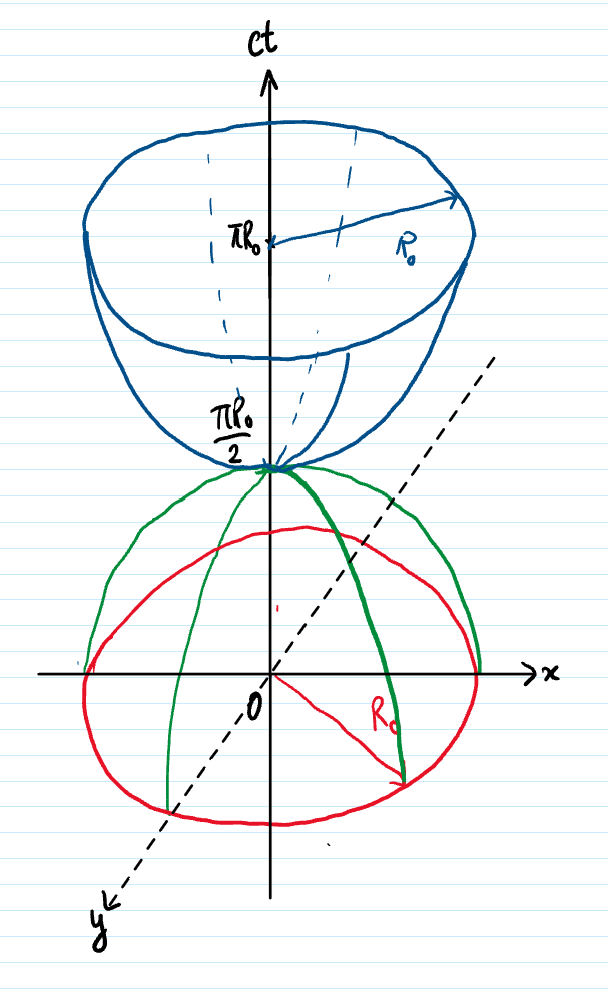
\includegraphics[height=0.7\textheight]{images/sketch6_7zwiebach.png}
    \caption{Sketch of the spacetime traced by the string in Zwiebach's 6.7}
    \label{fig: q6_7sol}
\end{figure}

\clearpage  
\section{Zwiebach's 7.4: Kasey's relativistic jumping rope}
Consider a relativistic open string with fixed endpoints: 
\begin{align}
    \vec{X}(t, 0) = \vec{x_1}, ~~~~~~ \vec{X}(t, \sigma_1) =\vec{x_2} \label{endpoints}
\end{align}
The boundary condition at $\sigma = 0$ is satisfied by the following solution to the wave equation: 
\begin{align}
    \vec{X}(t, \sigma) = \vec{x_1} + \frac{1}{2}\left(\vec{F}(ct + \sigma) - \vec{F}(ct - \sigma) \right) \label{sol_74}
\end{align}
Here $\vec{F}$ is a vector function of a single variable. 
\begin{enumerate} [(a)]
    \item Use (\ref{sol_74}) and the boundary condition at $\sigma = \sigma_1$ to find a condition on $\vec{F}(u)$.
    \item Write down the constraint on $\vec{F}(u)$ that arises from the parameterization conditions (7.42) 
    \begin{align*}
        \left( \frac{\partial \vec{X}}{\partial \sigma} \pm \frac{1}{c}\frac{\partial \vec{X}}{\partial t} \right)^2 =1 \tag{Zwiebach 7.42}
    \end{align*}
    As an application, consider Kasey's attempts to use a relativistic open string as a jumping rope. For this purpose, she holds the open string (in three spatial dimensions) with her right hand at the origin $\vec{x_1} = (0,0,0)$ and with her left hand at the point $z =L_0$ on the $z$ axis, or $\vec{x_2} = (0,0, L_0)$. As she starts jumping we observe that the tangent vector $\vec{X}'$ to the string at the origin rotates with constant angular velocity around the $z$ axis forming an angle $\gamma$ with it. 
    \item Use the above information to write an expression for $\vec{F}'(u)$. 
    \item Find $\sigma_1$ in terms of the length $L_0$ and the angle $\gamma$. 
    \item Calculate $\vec{X}(t, \sigma)$ for the motion of Kasey's relativistic jumping rope. 
    \item How is the energy distributed in the string as a function of $z$?
\end{enumerate}
\begin{figure}[ht]
    \centering
    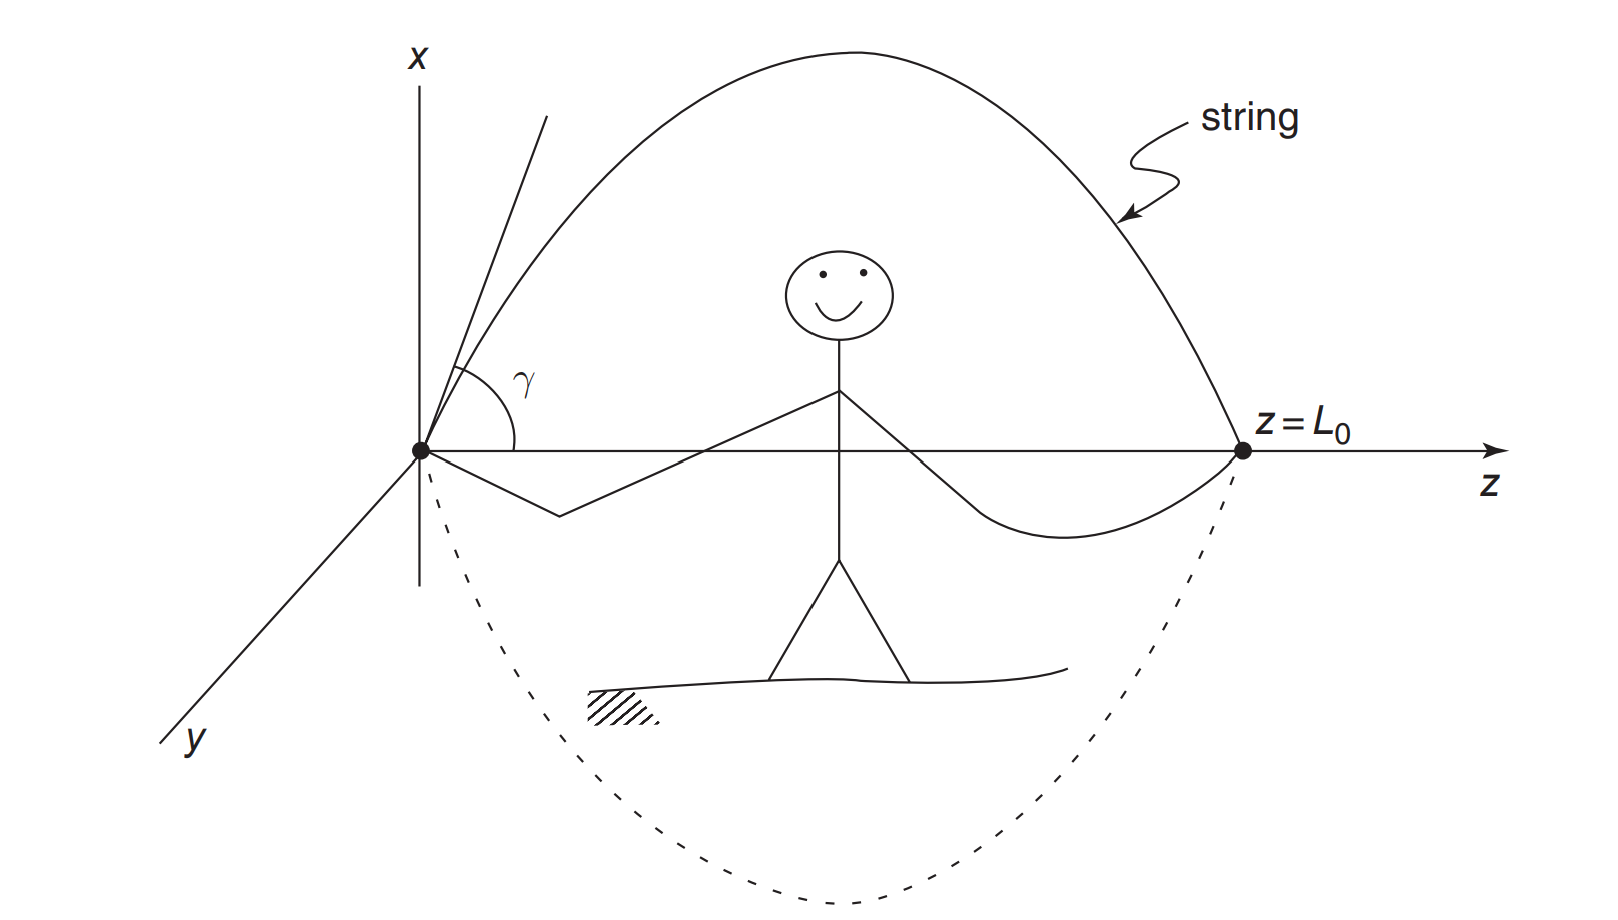
\includegraphics[width=0.6\linewidth]{images/q7_4 figure.png}
    \caption{Zwiebach's 7.4: Kasey's relativistic jumping rope}
    \label{fig: q7_4}
\end{figure}

\subsection*{Solution}
Note that we have omitted the vector signs over all variables. 
\begin{enumerate} [(a)]
    \item We have that 
    \begin{align*}
        {x_2} = {x_1} + \frac{1}{2}\left( {F}(ct + \sigma_1) - {F}(ct - \sigma_1) \right) 
    \end{align*}
    If we set $u = ct - \sigma_1$, we can rewrite the above equation as a recursive equation 
    \begin{align}
        F(u + 2\sigma_1) - F(u) = 2({x_2} - {x_1}) \label{F_periodic}
    \end{align}
    The most general form for $F(u)$ is then given by 
    \begin{align*}
        F(u) = G(u) + H(u) (x_2 - x_1) 
    \end{align*} 
    where $G(u)$ and $H(u)$ are arbitrary vector and scalar functions of $u$ respectively. The recursive condition imposes the following conditions on $G$ and $H$
    \begin{align*}
        G(u) = G(u + 2\sigma_1), ~~~~~~ H(u) = \frac{u}{\sigma_1}
    \end{align*}
    \item Note the derivatives of $X(t, \sigma)$ 
    \begin{align*}
        \frac{\partial X}{\partial t} = \frac{c}{2} \left( F'(ct + \sigma) - F'(ct - \sigma) \right) \\
        \frac{\partial X}{\partial \sigma} = \frac{1}{2} \left( F'(ct + \sigma) + F'(ct - \sigma) \right) 
    \end{align*}
    Imposing the parameterization conditions, we get 
    \begin{align*}
        [F'(ct + \sigma)]^2 = 1, ~~~~~~~~ [F'(ct - \sigma)]^2 = 1
    \end{align*}
    Since $\sigma$ takes on continuous values, we conclude that 
    \begin{align*}
        |F'(u)| = 1
    \end{align*}

    \item We are given that the string makes an angle $\gamma$ with the $z$ axis (as illustrated in Figure \ref{fig: q7_4}) and has angular velocity $\omega$. 
    
    Hence, 
    \begin{align}
        \frac{\partial X}{\partial \sigma} \bigg|_{\sigma = 0} = F'(ct) = (\sin \gamma \cos \omega t, \sin \gamma \sin \omega t, \cos \gamma) \notag \\
        \implies F'(u) = (\sin \gamma \cos \frac{\omega u}{c}, \sin \gamma \sin \frac{\omega u }{c}, \cos \gamma) \label{F'_eq}
    \end{align}

    \item By Eq. (\ref{F_periodic}), we must have that $F'(u)$ is $2\sigma_1$ periodic. In other words, we have the constraint
    \begin{align*}
        \cos \left(\frac{\omega u}{c}\right) &= \cos \left(\frac{\omega (u+2\sigma_1)}{c}\right) \\
        &= \cos \left( \frac{\omega u}{c} \right) \cos \left( \frac{2\omega \sigma_1}{c}\right) - \sin \left( \frac{\omega u}{c} \right) \sin \left( \frac{2\omega \sigma_1}{c}\right) \\
        &= \cos \left( \frac{\omega u}{c}\right) \tag{with $\sigma_1 = \dfrac{\pi c}{\omega}$ }
    \end{align*}
    which is satisfied when $\sigma_1 = \frac{\pi c}{\omega}$. We are given that 
    \begin{align*}
        F(2 \sigma_1) - F(0) = (0, 0, 2L_0)
    \end{align*}
    Consider the $z$-component of $F'(u)$. Note that 
    \begin{align*}
        \int_0^{2\sigma_1} F_z'(u) du = 2\sigma_1 \cos \gamma
    \end{align*}
    but we also have that 
    \begin{align*}
        \int_0^{2\sigma_1} F_z'(u) du = F_z(2\sigma_1) - F_z(0) = 2L_0
    \end{align*}
    which finally gives 
    \begin{align}
        \sigma_1 = \frac{L_0}{\cos \gamma } \label{sigma_1}
    \end{align}

    \item Integrating Eq. (\ref{F'_eq}) with respect to $u$ gives 
    \begin{align*}
        F(u) = \left( \frac{c}{\omega} \sin \gamma \sin \frac{\omega u}{c}, -\frac{c}{\omega} \sin \gamma \cos \frac{\omega u}{c}, u\cos \gamma \right)
    \end{align*}
    Recall the trigonometric identities 
    \begin{align*}
        \sin(a+b) - \sin(a-b) = 2\cos a \sin b \\
        \cos(a+b) - \cos(a-b) = -2 \sin a \sin b
    \end{align*}
    Given that $x_1 = (0,0,0)$, we can use Eq. (\ref{sol_74}) and the above identities to write 
    \begin{align*}
        X(t, \sigma) &= \frac{1}{2}[F(ct + \sigma) - F(ct - \sigma)] \\
        &= \frac{1}{2} \left( \frac{2c}{\omega} \sin \gamma \left(\cos \omega t  \sin \frac{\omega \sigma}{c} \right), \frac{2c}{\omega} \sin \gamma \left( \sin \omega t \sin \frac{\omega \sigma }{c} \right), 2\sigma \cos \gamma\right)
        % &= \frac{1}{2} \left( \frac{2\sigma_1}{\pi} \sin \gamma \left(\cos \frac{\pi ct}{\sigma_1}   \sin \frac{\pi \sigma}{\sigma_1} \right), \frac{2c}{\omega} \sin \gamma \left( \sin \omega t \sin \frac{\omega \sigma }{c} \right), 2\sigma \cos \gamma\right) 
    \end{align*}

    \item Consider 
    \begin{align*}
        dz &= \cos \gamma d\sigma \\
        &= \cos \gamma \frac{dE }{T_0 } \tag{Zwiebach 7.19} \\
        &= \frac{L_0}{\sigma_1} \frac{dE}{T_0} \tag{Eq. (\ref{sigma_1})}\\
        &= \frac{L_0}{E}dE \tag{Zwiebach 7.21} \\
        \implies \ln E &= \frac{z}{L_0} \implies E(z) = e^{z/L_0} 
    \end{align*}
\end{enumerate}

\newpage 

\section{Zwiebach's 9.3: Rotating open string in the light cone gauge}
\begin{enumerate} [(a)]
    \item From Zwiebach's Eq. (9.83), we know that 
    \begin{align*}
        M^2 = \frac{1}{\alpha'} \sum_{n=1}^\infty n \alpha_n^{I*} \alpha_n^I
    \end{align*}
    We are given $\alpha_1^I = (a, ia, 0, \cdots), \alpha_{-1}^I = (a, -ia, 0, \cdots)$ and $\alpha_n^I = 0$ for all other $n \in \Z$. Hence, 
    \begin{align*}
        M^2 = \frac{1}{\alpha'} 2a^2 \implies M = \sqrt{\frac{2}{\alpha'}} a 
    \end{align*}
    
    \item From Zwiebach's Eq. (9.69), we have 
    \begin{align*}
        X^I(\tau, \sigma) = x^I_0 + \sqrt{2\alpha' } \alpha^I_0 \tau + i \sqrt{2\alpha' }\sum_{n \neq 0} \frac{1}{n}\alpha^I_n e^{-in\tau} \cos n \sigma
    \end{align*}
    We are given that $x^I_0 = 0$ and that $\alpha_n^I = 0$ for all $n \neq 1,-1$. This leaves us with 
    \begin{align*}
        X^I(\tau, \sigma) &= i \sqrt{2\alpha' }\sum_{n \neq 0} \frac{1}{n}\alpha^I_n e^{-in\tau} \cos n \sigma \\
        &= i \sqrt{2\alpha'} \left(\alpha^I_1 e^{-i\tau} - \alpha^I_{-1} e^{i\tau}  \right) \cos\sigma
    \end{align*}
    This directly gives 
    \begin{align*}
        X^2(\tau, \sigma) &= i \sqrt{2\alpha'} a \left(e^{-i\tau} -  e^{i\tau} \right) \cos\sigma = 2 \sqrt{2\alpha'} a \sin\tau \cos \sigma \\
        X^3(\tau, \sigma) &=  -\sqrt{2\alpha'} a\left(e^{-i\tau} + e^{i\tau}  \right) \cos\sigma = -2\sqrt{2\alpha'} a \cos\tau \cos \sigma 
    \end{align*}
    Now, the length of the string is given by 
    \begin{align*}
        \ell &= 4a\sqrt{2\alpha'} 
    \end{align*}

    \item From Zwiebach's 9.77, we know that the transverse Virasoro modes $L_n^\perp$ are given by 
    \begin{align*}
        L_n^\perp = \frac{1}{2}\sum_{p \in \Z} \alpha_{n-p}^I \alpha_{p}^I 
    \end{align*}
    Since only $\alpha_1^I$ and $\alpha_{-1}^I$ are nonzero, the only potentially nonzero transverse Virasoro modes are $L_0^\perp$ and $L_{\pm 2}^\perp$. They are 
    \begin{align*}
        L_0^\perp &= \frac{1}{2} (\alpha_{-1}^I \alpha_1^I + \alpha_1^I \alpha_{-1}^I) = \frac{1}{2}(a^2 + a^2 + a^2 + a^2) = 2a^2 \\
        L_2^\perp &= \frac{1}{2} (\alpha^I_1)^2 = \frac{1}{2} (a^2 - a^2) = 0 \\
        L_{-2}^\perp &= \frac{1}{2}(\alpha_{-1}^I)^2 = \frac{1}{2} (a^2 -a^2) = 0 
    \end{align*}
    Finally, from Zwiebach's 9.80,
    \begin{align*}
        X^{-}(\tau, \sigma) &= x^-_0 + \frac{1}{p^+} L_0^\perp \tau + \frac{i}{p^+} \sum_{n \neq 0} \frac{1}{n} L_n^\perp e^{-in\tau} \cos n\sigma \\
        &= \frac{2a^2 \tau}{p^+} \tag{$x^-_0 = L_{n\neq 0}^\perp = 0$} 
    \end{align*}

    \item From Zwiebach's 9.62, we know that for open strings, 
    \begin{align*}
        X^+(\tau, \sigma) = 2\alpha' p^+ \tau 
    \end{align*}
    To have $X^1 = 0$, we must have that 
    \begin{align*}
        X^+ = X^- \implies \alpha' p^+ =  \frac{a^2}{p^+} \implies p^+ = \frac{a}{\sqrt{\alpha'}}
    \end{align*}
    With $X^1 = 0$, we have that $X^{\pm} = X^0/\sqrt{2} = t/\sqrt{2}$. This gives us a relation between $t$ and $\tau$:
    \begin{align*}
        t = 2\sqrt{2} \alpha' p^+ \tau = 2a\sqrt{2\alpha'} \tau 
    \end{align*}

    \item Zwiebach's 7.59 states that 
    \begin{align*}
        \ell = \frac{2c}{\omega } = \frac{2E}{\pi T_0}
    \end{align*}
    We know that 
    \begin{align*}
        \omega = \frac{\tau}{t} = \frac{1}{2a \sqrt{2\alpha'}}
    \end{align*}
    which allows us to verify 
    \begin{align*}
        \ell = 4a \sqrt{2\alpha'} = \frac{2}{\omega} 
    \end{align*}
    in natural units. From Zwiebach's 8.76, we also know that 
    \begin{align*}
        T_0 = \frac{1}{2\pi \alpha' } \implies \frac{\ell}{E} = 4\alpha' 
    \end{align*}
    which is true if we check with $E = M$ as above. 
\end{enumerate}


\newpage 
\section{Zwiebach's 10.6: Field equations and particle states for Kalb-Ramond field}
\begin{enumerate} [(a)]
    \item Let's swap the first two indices 
    \begin{align*}
        H_{\nu \mu \rho} &= \partial_\nu B_{\mu\rho} + \partial_\mu B_{\rho\nu} + \partial_\rho B_{\nu \mu} \\
        &= -\partial_\mu B_{\nu\rho} -\partial_\nu B_{\rho\mu} - \partial_\rho B_{\mu\nu } \\
        &= - H_{\mu\nu\rho}
    \end{align*}
    Similarly, we swap the last two indices 
    \begin{align*}
        H_{\mu \rho \nu} &= \partial_\mu B_{\rho\nu} + \partial_\rho B_{\nu\mu} + \partial_\nu B_{\mu \rho} \\
        &= -\partial_\mu B_{\nu\rho} -\partial_\nu B_{\rho\mu} - \partial_\rho B_{\mu\nu } \\
        &= - H_{\mu\nu\rho}
    \end{align*}
    Finally, the first and the third
    \begin{align*}
        H_{\rho \nu \mu} &= \partial_\rho B_{\nu\mu} + \partial_\nu B_{\mu\rho} + \partial_\mu B_{\rho \nu} \\
        &= -\partial_\mu B_{\nu\rho} -\partial_\nu B_{\rho\mu} - \partial_\rho B_{\mu\nu } \\
        &= - H_{\mu\nu\rho}
    \end{align*}
    showing that $H_{\mu\nu\rho}$ is totally antisymmetric. To prove that $H_{\mu\nu\rho}$ is invariant under the gauge transformation, we check 
    \begin{align*}
        \delta H_{\mu\nu\rho} &= \partial_\mu \delta B_{\nu\rho} +\partial_\nu \delta B_{\rho\mu} +\partial_\rho \delta B_{\mu\nu } \\
        &= \partial_\mu (\partial_\nu \epsilon_\rho - \partial_\rho \epsilon_\nu) + \partial_\nu (\partial_\rho \epsilon_\mu - \partial_\mu \epsilon_\rho) + \partial_\rho  (\partial_\mu \epsilon_\nu - \partial_\nu \epsilon_\mu)
    \end{align*}
    Since partials commute, the above expression goes to 0, as desired. 

    \item Using $\epsilon_\mu' = \epsilon_\mu + \partial_\mu \lambda$, we check 
    \begin{align*}
        \delta' B_{\mu\nu} &= \partial_\mu \epsilon_\nu' - \partial_\nu \epsilon_\mu'\\
        &= \partial_\mu (\epsilon_\nu + \partial_\nu \lambda) - \partial_\nu (\epsilon_\mu + \partial_\mu \lambda) \\
        &= \partial_\mu \epsilon_\nu - \partial_\nu \epsilon_\mu = \delta B_{\mu\nu}
    \end{align*}
    Hence, $\epsilon_\mu'$ and $\epsilon_\mu$ generate the same gauge transformation. 

    \item In momentum space, we have  
    \begin{align*}
        {\epsilon^\mu}'(p) = \epsilon^\mu (p) + ip^\mu \lambda(p) \\
        \implies {\epsilon^+}' (p) = {\epsilon^+} (p) + i{p^+} \lambda(p)
    \end{align*}
    and making the choice 
    \begin{align*}
        \lambda(p) &= i \frac{\epsilon^+(p)}{p^+} \implies {\epsilon^+}'(p) = 0 
    \end{align*}
    as desired. 

    \item We vary the action
    \begin{align*}
        \delta S &= -\frac{1}{3}\int d^D x \left(H^{\mu\nu\rho} \delta H_{\mu\nu\rho} \right) \\
        &= - \frac{1}{3} \int d^D x H^{\mu\nu\rho} (\partial_\mu \delta B_{\nu\rho} +\partial_\nu \delta B_{\rho\mu} +\partial_\rho \delta B_{\mu\nu }) \\
        &= - \int d^D x H^{\mu\nu\rho} \partial_\mu \delta B_{\nu \rho} \tag{reordering and relabelling}    
    \end{align*}
    Since we want this quantity to be 0 for all $\delta B_{\nu \rho}$, we need $\partial_\mu H^{\mu\nu\rho}$ to  be vanish
    \begin{align*}
        \partial_\mu H^{\mu\nu\rho} &= 0 \\
        \partial_\mu  (\partial^\mu B^{\nu\rho} + \partial^\nu B^{\rho\mu} + \partial^\rho B^{\mu\nu }) &= 0 
    \end{align*}
    In momentum space, this is 
    \begin{align*}
        p^2 B^{\nu \rho} + p_\mu p^\nu B^{\rho \mu } + p_\mu p^\rho B^{\mu \nu} = 0 
    \end{align*}

    \item By antisymmetry of $B^{\mu\nu}$, we have that $B^{++} = 0$. We want to choose $\epsilon^\mu(p)$ such that we also have $B^{+-} = B^{+I} = 0$.
    
    Since we have $\delta B^{\mu\nu} = \partial_\mu \epsilon_\nu - \partial_\nu \epsilon_\mu$, we know that 
    \begin{align*}
        \delta B^{++} &= 0 \\
        \delta B^{+-} &= \partial_+ \epsilon_- - \partial_- \epsilon_+ \\
        \delta B^{+I} &= \partial_+ \epsilon_I - \partial_I \epsilon_+ 
    \end{align*}
    Hence, we can take $\epsilon^+ = 0$ and then the equations above determine $\epsilon_-$ and $\epsilon_I$ completely. Now, the only non-zero field components are $B^{--}, B^{IJ}, B^{-I}$. 

    In this gauge, define $A^\mu = p_\nu B^{\mu\nu}$, which gives 
    \begin{align*}
        A^+ = 0, ~~~~~ A^- = p_I B^{-I} + p_- B^{--}, ~~~~~ A^I = p_J B^{IJ} + p_- B^{I-} 
    \end{align*}
    From the equation of motion derived in (d), we can now write
    \begin{align*}
        p^2 B^{\nu \rho } = -p^\nu A^\rho - p^\rho A^\nu 
    \end{align*}
    When $\nu \rho = +-$, we get $p^+ A^- = 0 \implies A^- = 0$

    When $ \nu \rho = +I$, we get $p^+ A^I = 0 \implies A^I = 0$. 

    Hence, $A^\mu = 0 \implies p^2 B^{\nu \rho} = 0$. 

    Finally, $A^- = 0 \implies B^{-I} \propto B^{--}$ and $A^I \implies B^{IJ} \propto B^{-J}$, implying that there is only one degree of freedom in the components of $B^{\mu\nu}$, namely $B^{-I}$. 

    \item Since each of the independent fields $B^{\mu\nu}$ can be expanded in terms of the oscillatory modes, we can write the one-particle states of the Kalb-Ramond field as 
    \begin{align*}
        \sum_{I,J=2}^{D-1} \xi_{IJ} a^{IJ \dagger}_p |\Omega \rangle 
    \end{align*}
    Since $a^{IJ\dagger} = - a^{JI\dagger}$, we conclude that $\xi_{IJ}$ is an antisymmetric matrix. 

\end{enumerate}

\newpage
\section{Zwiebach's 11.7: Transformations generated by light-cone gauge Lorentz generators $M^{+-}$ and $M^{-I}$}

It is useful to know the following commutation relations 
\begin{align*}
    [p^-, p^+] = [p^+, p^I] = [p^-, p^I] = 0 \\
    [x_0^-, p^I] = [x_0^-, x_0^I] = [p^+, x_0^I] = 0 \\
    [x_0^-, p^-] = i \frac{p^-}{p^+} \\
    [x_0^-, p^+] = -i \\
    [x_0^I, p^-] = i \frac{p^I}{p^+} \\
    [x_0^-, \frac{1}{p^+}] = \frac{i}{p^{+2}}
\end{align*}
\begin{enumerate}[(a)]
    \item $M^{+-}$ is given by 
    \begin{align*}
        M^{+-} = - \frac{1}{2}(x_0^- p^+ + p^+ x_0^-) = -x_0^- p^+ - \frac{1}{2}i 
    \end{align*}
    where we used $[x_0^-, p^+] = -i$ in the final step. Note that 
    \begin{align*}
        x^+ (\tau) = \frac{p^+ \tau }{m^2}, &~~~~ x^-(\tau) = x_0^- + \frac{p^- \tau }{m^2} \tag{Zwiebach's 11.63} \\
        x^I(\tau) &= x_0^I + \frac{p^I}{m^2}\tau \tag{Zwiebach's 11.15}
    \end{align*}
    Hence, the commutators of interest are 
    \begin{align*}
        [M^{+-}, x^+(\tau)] &= [-x_0^- p^+, \frac{p^+ \tau }{m^2}] = \frac{\tau }{m^2} (-x_0^- p^{+2} + p^+ x_0^- p^+) = i x^+(\tau) \\
        [M^{+-}, x^-(\tau)] &= [-x_0^- p^+, x_0^- + \frac{p^- \tau }{m^2}] \\
        &= x_0^-(-p^+ x_0^- + x_0^- p^+) +  \frac{\tau }{m^2} [-x_0^- p^+, p^-] \\
        &= -i x_0^- - \frac{\tau }{m^2} i \frac{p^-}{p^+} p^+ \\
        &= -i x^-(\tau) \\
        [M^{+-}, x^I(\tau)] &= [-x_0^- p^+, x^I_0 + \frac{p^I}{m^2}\tau ] =0 
    \end{align*}
    $M^{+-}$ generates a Lorentz transformation of these coordinates as follows 
    \begin{align*}
        \delta x^\mu = [-i\epsilon M^{+-}, x^\mu] \\
        \implies \delta x^+ = \epsilon x^+, \delta x^- = -\epsilon x^-, \delta x^I = 0 
    \end{align*}
    as expected.  

    \item $M^{-I}$ is defined as 
    \begin{align*}
        M^{-I} &= x_0^- p^I - \frac{1}{2} (x_0^I p^- + p^- x_0^I) \\
        &= x_0^- p^I - x_0^I p^- + \frac{1}{2}i \frac{p^I}{p^+}
    \end{align*}
    Hence, the commutators of interest are 
    \begin{align*}
        [M^{-I}, x^+(\tau)] &= \left[x_0^- p^I - x_0^I p^- + \frac{1}{2}i \frac{p^I}{p^+}, \frac{p^+ \tau }{m^2}\right] \\
        &= \frac{\tau }{m^2} [x_0^- p^I, p^+] \\
        &= -i \frac{\tau p^I}{m^2} \\
        &= i (x_0^I - x^I) \\
        [M^{-I}, x^- (\tau)] &= \left[x_0^- p^I - x_0^I p^- + \frac{1}{2}i \frac{p^I}{p^+}, x_0^- + \frac{p^- \tau }{m^2}\right] \\
        &= -x_0^I[ p^-, x_0^-] + \frac{1}{2}i [\frac{p^I}{p^+}, x_0^-] + \frac{\tau }{m^2} \left( [x_0^-, p^-] p^I + [-x_0^I, p^-] p^- \right) \\
        &= i x_0^I \frac{p^-}{p^+} + \frac{1}{2} \frac{1}{p^{+2}} p^I + \frac{\tau}{m^2} \left( i \frac{p^-}{p^+} p^I - i \frac{p^I}{p^+}p^- \right) \\
        &= \frac{1}{p^+} \left( ix_0^I p^- + \frac{p^I}{2p^+} \right) \\
        [M^{-I}, x^J(\tau)] &= \left[x_0^- p^I - x_0^I p^- + \frac{1}{2}i \frac{p^I}{p^+}, x_0^J + \frac{p^J}{m^2} \tau \right] \\
        &= x_0^- [p^I, x_0^J] - x_0^I [p^-, x_0^J ] + \frac{i}{2} [p^I, x_0^J] \frac{1}{p^+} - \frac{\tau}{m^2}[x_0^I, p^J] p^- \\
        &= -i x_0^- \delta_{IJ} + ix_0^I \frac{p^J}{p^+} + \frac{1}{2p^+} \delta_{IJ} - i\frac{\tau }{m^2} \delta_{IJ} p^- \\
        &= -i \delta_{IJ} x^-(\tau) + \frac{1}{p^+} \left( ix_0^I p^J + \frac{\delta_{IJ}}{2} \right)   
    \end{align*}
    We know that the expected Lorentz transformations are 
    \begin{align*}
        [M^{-I}, x^+(\tau)] &= -ix^I(\tau) \tag{11.80} \\
        [M^{-I}, x^-(\tau)] &= 0 \\
        [M^{-I}, x^I(\tau)] &= -i \delta_{IJ}x^-(\tau) 
    \end{align*}
    Note that these differ from our results above by exactly the following term in each case 
    \begin{align*}
        \frac{im^2}{2} \left( \frac{x_0^I}{p^+} \frac{dx^\mu}{d\tau} + \frac{dx^\mu}{d\tau} \frac{x_0^I }{p^+} \right) 
    \end{align*}
    which corresponds to a reparameterization by 
    \begin{align*}
        \lambda = \frac{im^2 x_0^I}{p^+}
    \end{align*}
\end{enumerate}


\newpage 
\section{Zwiebach's 12.10: Reparameterization and constraints}
\begin{enumerate} [(a)]
    \item Check 
    \begin{align*}
        \dot{\xi^\tau} &= me^{im\tau } \cos m\sigma = {\xi^\sigma} ' \\
        \dot{\xi^\sigma} &= im e^{im \tau} \sin m \sigma = {\xi^\tau} ' 
    \end{align*}

    \item First note that 
    \begin{align*}
        \frac{d \tau }{d \tau '} = 1 - \epsilon \dot{\xi}^\tau, ~~~~ \frac{d \tau }{d \sigma '} = - \epsilon {\xi^\tau} ', ~~~~ \frac{d \sigma }{d \sigma '} = 1- \epsilon {\xi^\sigma} ', ~~~~ \frac{d\sigma}{d \tau'} = - \epsilon \dot{\xi}^\sigma 
    \end{align*}
    Check that 
    \begin{align*}
        \frac{\partial X}{\partial \tau '} &= \frac{\partial X}{\partial \tau }\frac{\partial \tau}{\partial \tau '} +\frac{\partial X}{\partial \sigma } \frac{\partial \sigma }{\partial\tau'} = \frac{\partial X}{\partial \tau} - \epsilon \left( \frac{\partial X}{\partial \tau} \dot{\xi}^\tau + \frac{\partial X}{\partial \sigma} \dot{\xi}^\sigma \right) \\
        \frac{\partial X}{\partial \sigma '} &= \frac{\partial X}{\partial \tau}\frac{\partial \tau }{\partial \sigma'} + \frac{\partial X}{\partial \sigma} \frac{\partial \sigma }{\partial \sigma'} =  \frac{\partial X}{\partial \sigma} - \epsilon \left( \frac{\partial X}{\partial \tau} {\xi^\tau}' + \frac{\partial X}{\partial \sigma} {\xi^\sigma}' \right)
    \end{align*}
    Using results from part (a), we can write 
    \begin{align*}
        \frac{\partial X}{\partial \tau '} \pm \frac{\partial X}{\partial \sigma '} &= \frac{\partial X}{\partial \tau} \pm \frac{\partial X}{\partial \sigma} - \epsilon \left[ \left( \frac{\partial X}{\partial \tau} \pm \frac{\partial X}{\partial \sigma } \right) \dot{\xi}^\tau + \left( \frac{\partial X}{\partial \sigma} \pm \frac{\partial X}{\partial \tau } \right) \dot{\xi}^\sigma \right] \\
        &= \left( \frac{\partial X}{\partial \sigma} \pm \frac{\partial X}{\partial \tau } \right) \left( 1 - \epsilon \dot{\xi}^\tau - \epsilon \dot{\xi}^\sigma \right)
    \end{align*}
    Now, see that the classical constraints yield
    \begin{align*}
        \left( \frac{\partial X}{\partial \tau '} \pm \frac{\partial X}{\partial \sigma '} \right)^2 = \left( \frac{\partial X}{\partial \sigma} \pm \frac{\partial X}{\partial \tau } \right)^2 \left( 1 - \epsilon \dot{\xi}^\tau - \epsilon \dot{\xi}^\sigma \right)^2 = 0 
    \end{align*}
    from which the constraints in the $(\tau', \sigma')$ coordinates follow (by adding and subtracting the $\pm$ terms from each other). 
\end{enumerate}




\newpage 
\section{Zwiebach's 13.5: Unoriented closed strings}
\begin{enumerate} [(a)]
    \item The following image shows how the first and second strings are related to each other. 
    \begin{center}
        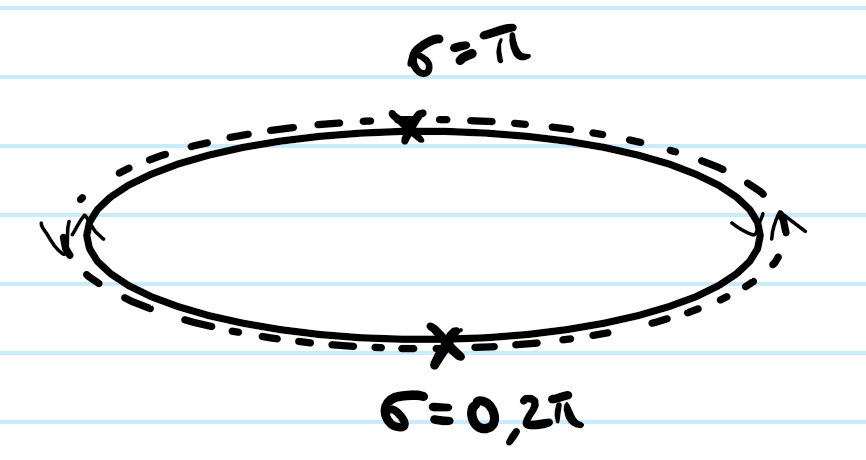
\includegraphics[width=7cm]{images/13_5a.png}
    \end{center}
    \item Zwiebach's 13.24 gives 
    \begin{align*}
        X^\mu(\tau, \sigma) = x^\mu_0 + \sqrt{2\alpha'} \alpha^\mu_0 \tau + i \sqrt{\frac{\alpha'}{2}} \sum_{n\neq 0} \frac{e^{-in\tau}}{n} (\alpha_n^\mu e^{in\sigma} + \overline{\alpha}_n^\mu e^{-in\sigma})
    \end{align*}
    Since $\sigma$ only occurs in the exponential terms at the end, we can immediately conclude 
    \begin{align*}
        \Omega x_0^I \Omega^{-1} = x_0^I, ~~~~~\Omega \alpha_0^I \Omega^{-1} = \alpha_0^I 
    \end{align*}
    Using the identity $e^{\pm in(2\pi - \sigma)} = e^{\mp in \sigma}$ then gives 
    \begin{align*}
        \Omega \alpha_n^I \Omega^{-1} = \overline{\alpha}_n^I, ~~~~~~~ \Omega \overline{\alpha}_n^I \Omega^{-1} = \alpha_n^I 
    \end{align*} 
    
    \item From Zwiebach's 13.24, we have 
    \begin{align*}
        X^-(\tau, \sigma) = x^-_0 + \sqrt{2\alpha'} \alpha^-_0 \tau + i \sqrt{\frac{\alpha'}{2}} \sum_{n\neq 0} \frac{e^{-in\tau}}{n} (\alpha_n^- e^{in\sigma} + \overline{\alpha}_n^- e^{-in\sigma})
    \end{align*}
    Using Zwiebach's 13.37 and 13.40, we can write 
    \begin{align*}
        \overline{\alpha}_n^- = \frac{1}{p^+ \sqrt{2\alpha'}} \sum_{p \in \mathbb{Z}} \overline{\alpha}_p^I \overline{\alpha}_{n-p}^I, ~~~~~~ \alpha_n^- = \frac{1}{p^+ \sqrt{2\alpha'}} \sum_{p \in\mathbb{Z}} \alpha_p^I \alpha_{n-p}^I 
    \end{align*}
    which, when we use (b), immediately gives us 
    \begin{align*}
        \Omega \overline{\alpha}_n^- \Omega^{-1} = \alpha_n^-, ~~~~~ \Omega \alpha_n^- \Omega^{-1} = \overline{\alpha}_n^- 
    \end{align*}
    Moreover, Zwiebach's 13.41 tells us that 
    \begin{align*}
        \alpha_0^- = \overline{\alpha}_0^- \implies \Omega \alpha_0^- \Omega^{-1} = \alpha_0^- 
    \end{align*}
    With our assumption that $\Omega x_0^- \Omega^{-1}$, we have our desired $\Omega X^-(\tau, \sigma) \Omega^{-1} = X^-(\tau, 2\pi - \sigma)$. 

    Since the Hamiltonian for the closed string is given as 
    \begin{align*}
        H = L_0^\perp + \overline{L}_0^\perp - 2
    \end{align*}
    it does not change under action of the twist operator and we say that orientation reversal is a symmetry of closed string theory. 

    \item When $N^\perp = \overline{N}^\perp = 0$, the only state in the state space is $| p^+, \vec{p}_T \rangle$. Since there is only one state, the twist eigenvalue is $+1$. 
    
    When $N^\perp = \overline{N}^\perp = 1$, Zwiebach's 13.64 gives the general form of the state as 
    \begin{align*}
        \sum_{I,J} R_{IJ} a^{I\dagger}_1 \overline{a}^{J\dagger} |p^+, \vec{p}_T \rangle 
    \end{align*}
    Under action of the twist operator, the barred and unbarred raising operators get swapped and $R_{IJ} \to R_{JI}$. If we write $R_{IJ}$ as in Zwiebach's 13.65, 
    \begin{align*}
        R_{IJ} = S_{IJ} + A_{IJ}
    \end{align*}
    then the symmetric states have eigenvalue $+1$ while the antisymmetric states have eigenvalue $-1$. 

    When $N^\perp = \overline{N}^\perp = 2$, there are three distinct contributions to the state space: 
    \begin{align*}
        &\sum_{I,J} R_{I,J} a_2^{I, \dagger} \overline{a}_2^{J, \dagger} |p^+, \vec{p}_T \rangle \\
        &\sum_{IJK} \left[R_{I,JK}a_2^{I \dagger} \overline{a}_1^{J \dagger}\overline{a}_1^{K \dagger} + \overline{R}_{I, JK}\overline{a}_2^{I \dagger} {a}_1^{J \dagger} {a}_1^{K \dagger} \right] |p^+, \vec{p}_T \rangle  \\
        &\sum_{IJKL} R_{IJ, KL}a_1^{I\dagger}a_1^{J\dagger}\overline{a}_1^{K\dagger} \overline{a}_1^{L\dagger} |p^+, \vec{p}_T \rangle
    \end{align*}
    In each case, we have a square matrix which can be decomposed into a sum of its symmetric and antisymmetric parts. Hence, as in the $N^\perp = 1$ case, we have eigenvalue $+1$ for the symmetric states and $-1$ for the antisymmetric states. 

    To obtain the unoriented theory, we would have to discard the eigenvalue $-1$ states. Hence, the massless fields are the graviton and the dilaton only. 
\end{enumerate}


\section{Zwiebach's 14.3: Massive level in the open superstring}
\begin{enumerate} [(a)]
    \item We need to count all possible choices of $b_i$'s such that there are no repetitions. We know that ordering does not matter because one list of $b_i$'s only differs from another reordered list of the same $b_i$'s by a constant factor. 
    
    Hence, the number of inequivalent $b^{i_1} b^{i_2}$'s is $8C2 = 28$. 

    The number of inequivalent $b^{i_1}b^{i_2}b^{i_3}$'s is $8C3 = 56$. 
    
    The number of inequivalent $b^{i_1}b^{i_2}b^{i_3}b^{i_4}$'s is $8C4 = 70$. 

    \item Consider $\alpha' M^2 = 1$. For the NS sector, we have 
    \begin{align*}
        \alpha' M^2 = N^\perp - \frac{1}{2}
    \end{align*}
    Hence, we get $N^\perp = 3/2$. From Zwiebach's 14.38, we know that there are three states that contribute to the NS sector; they are 
    \begin{align*}
        \{ \alpha_{-1}^I b_{-1/2}^J, b^I_{-3/2}, b^I_{-1/2}, b^J_{-1/2}, b^K_{-1/2} \} |NS\rangle 
    \end{align*}
    They contribute (respectively) $8 \times 8 + 8 + 56 = 128$ states in total. 

    For the R sector, we have 
    \begin{align*}
        \alpha' M^2 = N^\perp 
    \end{align*}
    Hence, we get $N^\perp = 1$. From Zwiebach's 14.54, there are two ways to construct such (fermionic) states 
    \begin{align*}
        \{ \alpha_{-1}^I, d_{-1}^I \} |R_a \rangle 
    \end{align*}
    They contribute (respectively) $8 \times 8 + 8 \times 8 = 128$ states (there are 8 $|R_a\rangle$ states) in total, which agrees with the NS sector. 

    Now consider $\alpha' M = 2$. For the NS sector, we get $N^\perp = 5/2$. There are 7 ways to construct the contributing states 
    \begin{align*}
        \{ \alpha_{-2}^I b^J_{-1/2}, \alpha_{-1}^I \alpha_{-1}^J b^K_{-1/2}, \alpha_{-1}^I b^J_{-1/2}b^K_{-1/2}b^L_{-1/2}, \alpha_{-1}^I b^J_{-3/2}, \\
        b_{-1/2}^Ib_{-1/2}^Jb_{-1/2}^Kb_{-1/2}^Lb_{-1/2}^M, b_{-3/2}^I b_{-1/2}^J b_{-1/2}^K, b_{-5/2}^I\} |NS \rangle 
    \end{align*}
    They contribute $(8 \times 8) + (28 \times 8) + (8 \times 56) + (8 \times 8) + 8C5 + (8 \times 28) + 8 = 1088$ states. 

    For the $R$ sector, we get $N^\perp = 2$. From Zweibach's 14.54, there are 5 ways to construct the contributing states
    \begin{align*}
        \{\alpha_{-2}^I, \alpha_{-1}^I \alpha_{-1}^J, d_{-1}^I, d_{-1}^J \} |R_a \rangle \\
        \{ \alpha_{-1}^I d_{-1}^J, d_{-2}^I \}  |R_{\overline{a}} \rangle 
    \end{align*}
    They contribute $8 \times (8 + 28 + 28 + 8\times8 + 8) = 1088$ states in total, as desired. 
\end{enumerate}
\end{document}  